\section{Predictive Analysis}
\subsection{Data Preparation}
Our goal is to classify the players in two categories: 'strong' players and the 'weak' players.
To do this, we started from the dataframe of the players used in the clustering phase and we labeled them in the two aforementioned classes, exploiting the rank of each player. We decided that the players whose rank fall in a category that is top 5, top 10, top 25, top 50 or top 100 are labelled as strong, thus, all the others as 'weak'. For the male players, we also label as 'strong' the one whose rank is 'top 250'.

Furthermore, we removed some features that we considered irrelevant, such as the players' hand obtained previously through a sampling process and the win rates on different surfaces, but keeping the average number of wins for each surface. Furthermore, we also didn't care about the players' nationality because it's useless for the classification purpose (a player's nationality can't determine his actual strength).

Finally, we removed the rank range, ranking points and ranking, to ensure that the classifier doesn't learn our labeling strategy.

\textit{The classification was done by dividing the male players from the female ones}, this means that there are some models trained using the 'male' data set that work only with the male players data and other ones that work with the female one.
Initially, we conducted the classification analysis by using our entire dataset which is made by both male and female players, the latter are present in minority, about 32\% of the entire data set. By doing in this way the classification metrics were good, but this happened due to the fact that our data set is imbalanced with respect to the players' sex. In fact, we tried to build two test sets based on the players' sex and we discovered that the classification models worked well on the 'male' set, while their performance dropped down on the 'female' set. For this reason, we present our analysis for this section by keeping male and female players separated.

\subsection{Imbalanced data}
Our labeling strategy carried out an imbalanced data set, which is likely to happen in competitive sports. The problem is that the classifiers trained on imbalanced data sets can perform bad as they tend to overfit towards the majority class. In our case, the male dataset has a distribution of the 'strong' and 'weak' players which is circa 74\% and 26\% respectively, totalling 1102 players. The female data set is also imbalanced to the 'weak' class, having a 76/24 percentage distribution, totalling 498 players. To overcome this problems we exploited the SMOTE approach for over-sampling the minority class combined with an under-sampling on the majority class. In this way the distribution of the players is 55\% for the 'weak' class and 45\% for the 'strong' one.

\subsection{Classification methods}
Before applying any of the following classification algorithms, we splitted the dataset into development and test sets, the latter consisting of 10\% of the original data set. Furthermore we used the StandardScaler algorithm from the scikit-learn library to standardize our data.

The following results have been obtained by exploiting the best parameters carried out by the K-Fold cross validation, with K equal to 4, comparing the results by measuring the accuracy score between the K folds. For the lack of space, we will only show the graphical results for the male players, whereas in \autoref{subsect:comparison} we study the performance obtained by our models in both the male and female data set.

\paragraph{Evaluation} In order to evaluate the goodness of our models, we'll show classification metrics like accuracy, precision, recall and F1 score. The miss-classified patterns can be numerically viewed by using the confusion matrix (label 0 for 'weak', 1 for 'strong') and graphically by plotting the ROC curve. Finally, for those models that are interpretable, we'll show the "global" weight that each feature had in the classification of the tennis players. Talking about the test set, it is made up of imbalanced data, having the same distribution as the original dataset, thus it's without any sampling strategy applied. This means that any of the following algorithm must beat the dummy classifier.


\subsubsection{Decision tree}
Decision tree is a classification method which produces interpretable results. It's not one of the best algorithms we tested, but, anyway, its performances are pretty good.
\begin{figure}[H]
    \centering
    \subfloat[Confusion matrix]{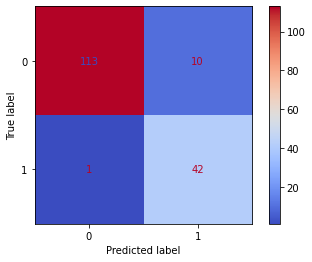
\includegraphics[width=0.28\linewidth]{images/predictive_analysis/dec_tree/tree_conf_m.png}}
    \subfloat[Features importance]{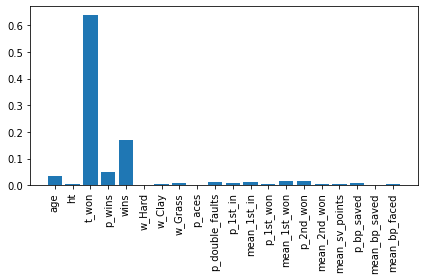
\includegraphics[width=0.35\linewidth]{images/predictive_analysis/dec_tree/tree_imp_m.png}}
    \subfloat[ROC curve]{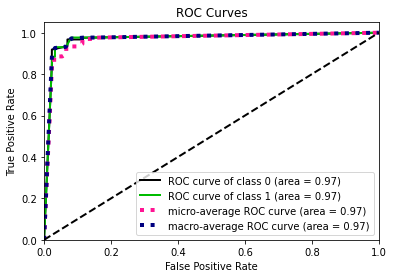
\includegraphics[width=0.35\linewidth]{images/predictive_analysis/dec_tree/tree_roc_m.png}}\\
    \subfloat[Decion tree splitting]{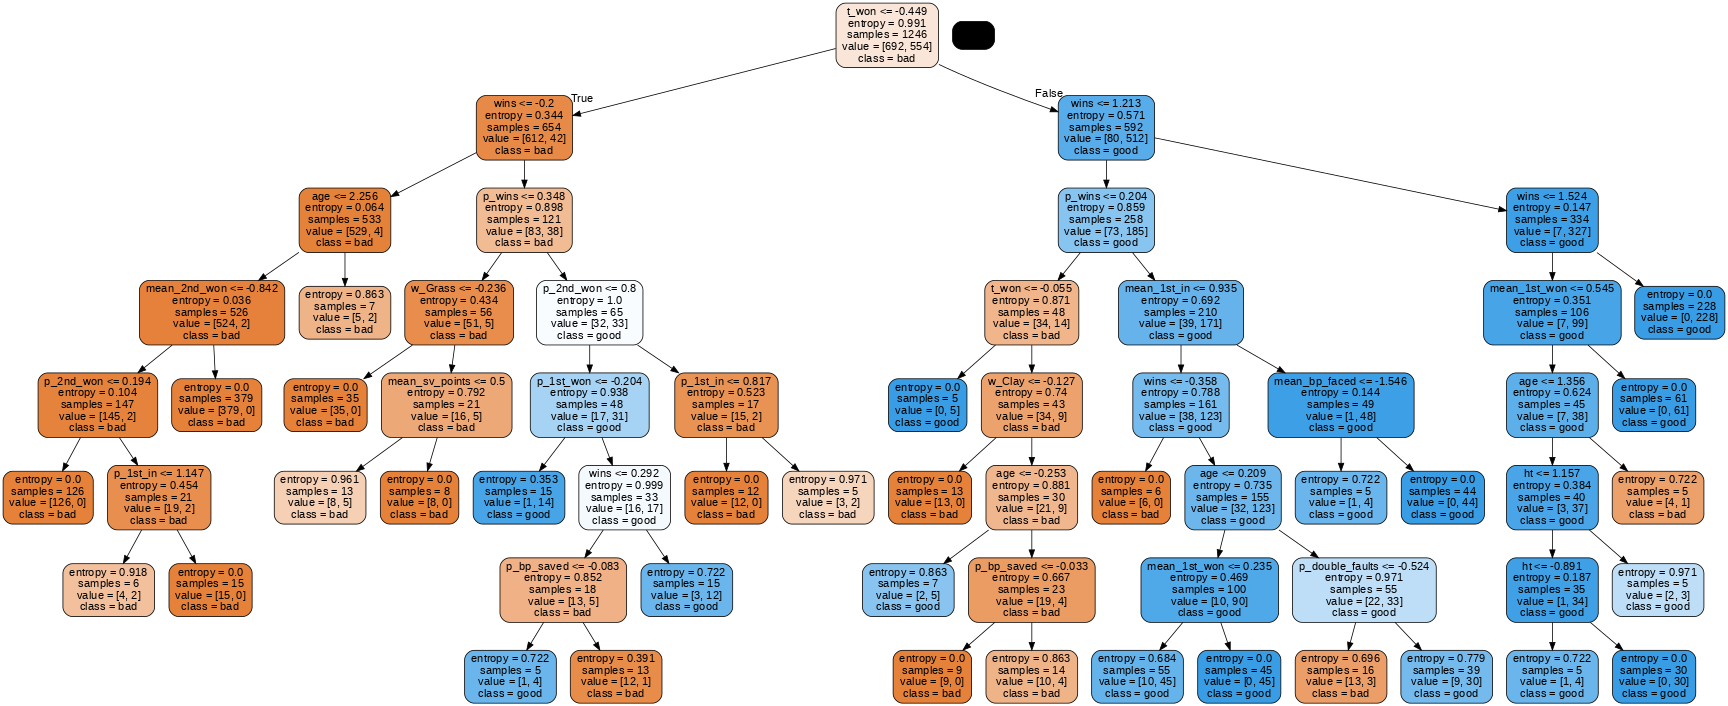
\includegraphics[width=0.8\linewidth]{images/predictive_analysis/dec_tree/tree_plot.png}}
    \caption{Results for the Decision Tree classifier}
    \label{fig:DTResults}
\end{figure}

\subsubsection{Naive Bayes}
The Naive Bayes classifier is a "probabilistic classifier" based on applying Bayes' theorem with strong (naïve) independence assumptions between the features.
\begin{figure}[H]
    \centering
    \subfloat[Confusion matrix]{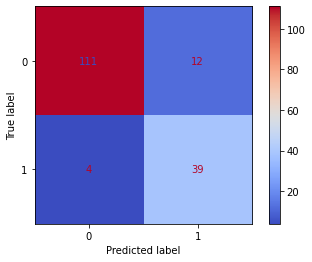
\includegraphics[width=0.28\linewidth]{images/predictive_analysis/naive_bayes/naive_conf_m.png}}
    \subfloat[ROC curve]{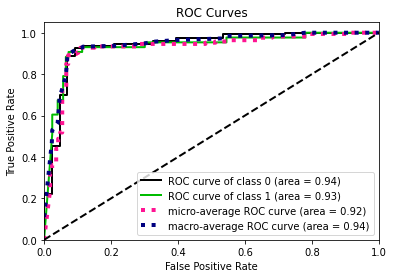
\includegraphics[width=0.35\linewidth]{images/predictive_analysis/naive_bayes/naive_roc_m.png}}
    \caption{Results for the Naive Bayes classifier}
    \label{fig:NBResults}
\end{figure}

\subsubsection{Random forest}
It's an ensemble method specifically designed for decision trees, it combines the predictions made by multiple decision trees and outputs the class that is the mode of the class' output by individual trees.
\begin{figure}[H]
    \centering
    \subfloat[Confusion matrix]{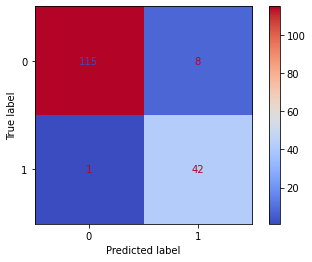
\includegraphics[width=0.28\linewidth]{images/predictive_analysis/rand_forest/rf_conf_m.png}}
    \subfloat[Features importance]{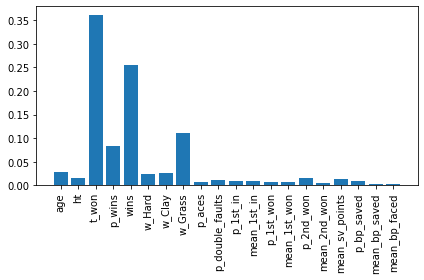
\includegraphics[width=0.35\linewidth]{images/predictive_analysis/rand_forest/rf_imp_m.png}}
    \subfloat[ROC curve]{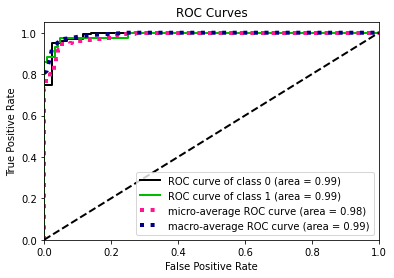
\includegraphics[width=0.35\linewidth]{images/predictive_analysis/rand_forest/rf_roc_m.png}}
    \caption{Results for the Random Forest classifier}
    \label{fig:RFResults}
\end{figure}

\subsubsection{Adaptive boosting (AdaBoost)}
It can be used as ensembler of based classifiers to improve performance. The output of the base learning algorithms ('weak learners') is combined into a weighted sum that represents the final output of the boosted classifier. AdaBoost is adaptive in the sense that subsequent weak learners are tweaked in favor of those instances misclassified by previous classifiers.
\begin{figure}[H]
    \centering
    \subfloat[Confusion matrix]{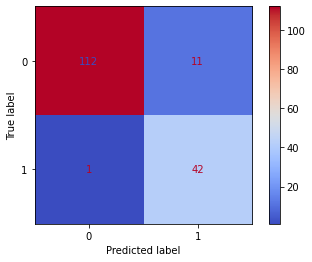
\includegraphics[width=0.28\linewidth]{images/predictive_analysis/ada_boost/ada_conf_m.png}}
    \subfloat[Features importance]{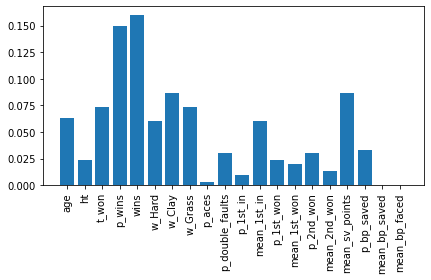
\includegraphics[width=0.35\linewidth]{images/predictive_analysis/ada_boost/ada_imp_m.png}}
    \subfloat[ROC curve]{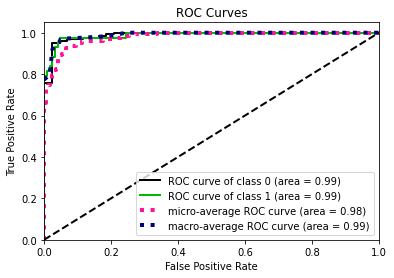
\includegraphics[width=0.35\linewidth]{images/predictive_analysis/ada_boost/ada_roc_m.png}}
    \caption{Results for the AdaBoost classifier}
    \label{fig:AdaBoostResults}
\end{figure}

\subsubsection{Rule based}
The rule-based classifier is a classification scheme that makes use of IF-THEN rules for class prediction. 
\begin{figure}[H]
    \centering
    \subfloat[Confusion matrix]{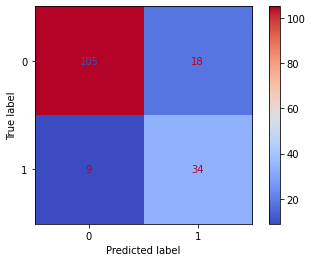
\includegraphics[width=0.28\linewidth]{images/predictive_analysis/rule_based/rule_conf_m.png}}
    \subfloat[ROC curve]{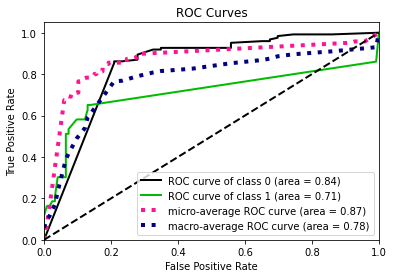
\includegraphics[width=0.35\linewidth]{images/predictive_analysis/rule_based/rule_roc_m.png}}
    \caption{Results for the Rule Based classifier}
    \label{fig:RBResults}
\end{figure}

\subsubsection{K-nearest neighbors (KNN)}
The KNN is an instance based classifier, it uses class labels of nearest neighbors to determine the class label of unknown records.
\begin{figure}[H]
    \centering
    \subfloat[Confusion matrix]{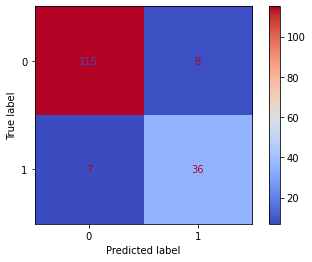
\includegraphics[width=0.28\linewidth]{images/predictive_analysis/knn/knn_conf_m.png}}
    \subfloat[ROC curve]{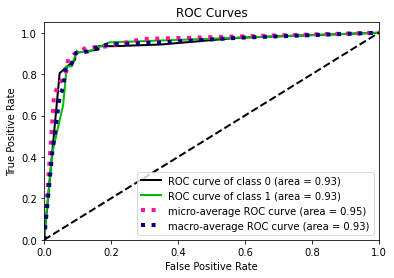
\includegraphics[width=0.35\linewidth]{images/predictive_analysis/knn/knn_roc_m.png}}
    \caption{Results for the KNN classifier}
    \label{fig:KNNResults}
\end{figure}

\subsubsection{Support-vector machine (SVM)}
SVM is a robust classifier based on statistical learning frameworks, it maps training examples to points in space to maximise the width of the gap between the two categories. New examples are then mapped into that same space and predicted to belong to a category based on which side of the gap they fall.
\begin{figure}[H]
    \centering
    \subfloat[Confusion matrix]{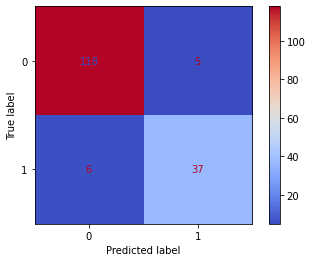
\includegraphics[width=0.28\linewidth]{images/predictive_analysis/svm/svm_conf_m.png}}
    \subfloat[ROC curve]{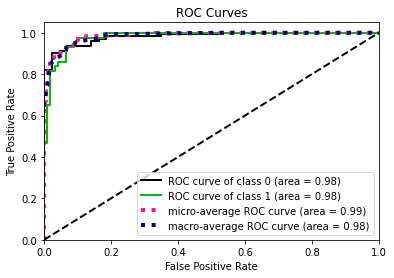
\includegraphics[width=0.35\linewidth]{images/predictive_analysis/svm/svm_roc_m.png}}
    \caption{Results for the SVM classifier}
    \label{fig:SVMResults}
\end{figure}

\subsubsection{Neural network}
We developed a FF neural network made up of two hidden layers whose neurons are 'activated' by the elu function and a softmax on the output layer. To ensure the generalization capability, we use the dropout technique and the layer normalization, to stabilize the training phase. In the end, we used the categorical cross entropy as loss function.
\begin{figure}[H]
    \centering
    \subfloat[Confusion matrix]{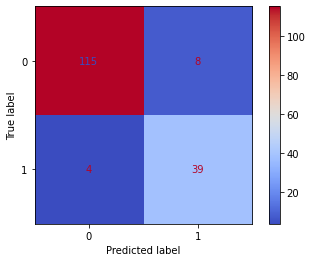
\includegraphics[width=0.28\linewidth]{images/predictive_analysis/nn/nn_conf_m.png}}
    \subfloat[Learning curve]{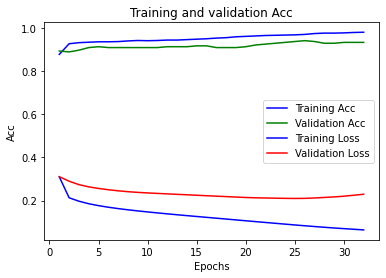
\includegraphics[width=0.35\linewidth]{images/predictive_analysis/nn/nn_learnCurve_m.png}}
    \subfloat[ROC curve]{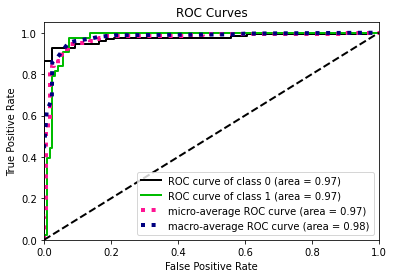
\includegraphics[width=0.35\linewidth]{images/predictive_analysis/nn/nn_roc_m.png}}
    \caption{Results for the Neural Network classifier}
    \label{fig:NNResults}
\end{figure}

\subsubsection{TabNet}
TabNet \cite{arik2020tabnet} is a novel high-performance and interpretable canonical deep tabular data learning architecture. TabNet uses sequential attention to choose which features to reason from at each decision step, enabling interpretability and more efficient learning as the learning capacity is used for the most salient features.
\begin{figure}[H]
    \centering
    \subfloat[Global feature importance]{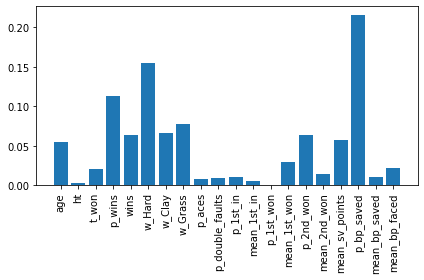
\includegraphics[width=0.35\linewidth]{images/predictive_analysis/tab_net/tab_imp_m.png}}
    \subfloat[Local feature importance]{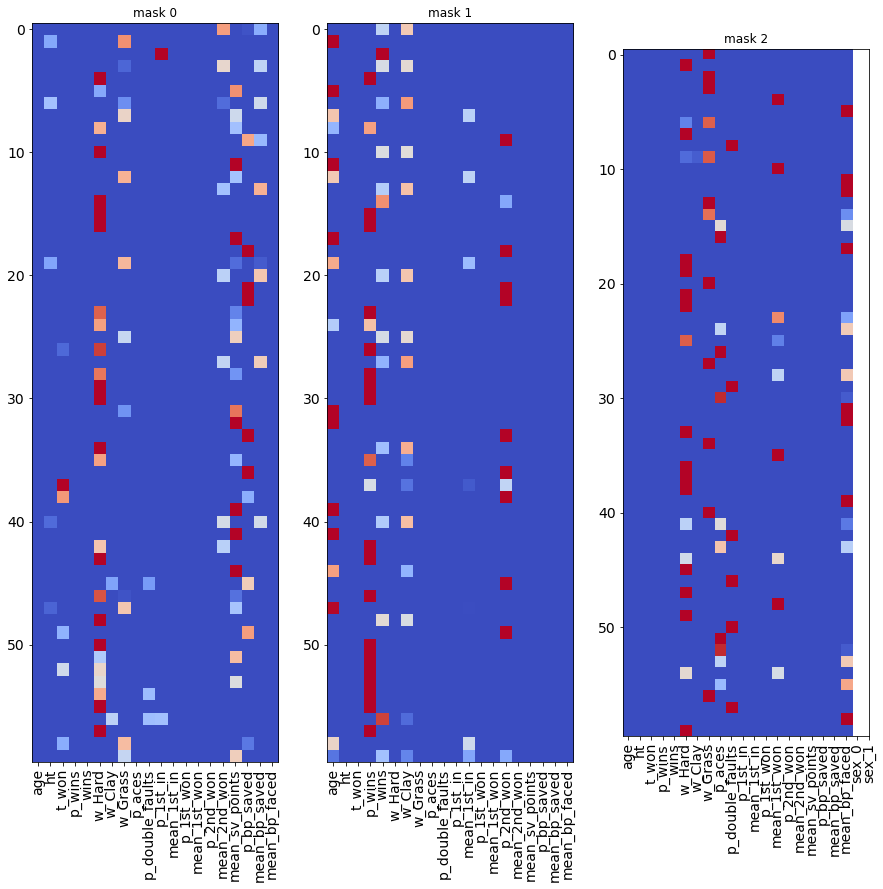
\includegraphics[width=0.33\linewidth]{images/predictive_analysis/tab_net/tab_impLoc_m.png}}
    \subfloat[ROC curve]{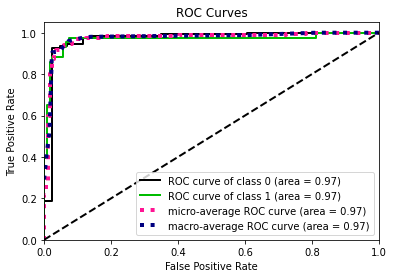
\includegraphics[width=0.30\linewidth]{images/predictive_analysis/tab_net/tab_roc_m.png}}
    \caption{Results for the Tab Net classifier}
    \label{fig:TNResults}
\end{figure}

\subsection{Comparison} \label{subsect:comparison}
In this section we show how the aforementioned algorithms performed in both the male and female datasets. In \autoref{tab:female_compare} and \autoref{tab:male_compare} we reported the performances in percentages. For each numerical entry, the first number is referred to the 'weak' class and the second one to the 'strong' class. In general, there wasn't a model that performed well in both the two data set as AdaBoost obtained the best performance on the female data set, whereas Random Forest in the male one. In the end, we can assert that AdaBoost was the best model overall, which is a good result because it is also interpretable. For this reason, we also compared the feature importance that this model associates to the male players with respect to the female players, as shown in \autoref{fig:FeatImpSex}.

\begin{table}[H]
\footnotesize
\centering
%\tiny
\begin{tabular}{c|c|c|c|c|c|c|c|c}\hline \hline
\multicolumn{9}{c}{\textbf{Female players classification}}\\ \hline \hline
\multirow{2}{*}{\textbf{Model}} & \multicolumn{4}{c|}{\textbf{Training}} & \multicolumn{4}{c}{\textbf{Test}} \\\cline{2-9}
& Prec. & Rec. & F1 & Acc. & Prec. & Rec. & F1 & Acc. \\\hline
Decision Tree & 95/89 & 91/94 & 93/91 & 92 & 96/62 & 82/89 & 89/73 & 84 \\
Naive Bayes & 91/84 & 86/90 & 89/87 & 88 & 96/62 & 82/89 & 89/73 & 84\\
\rowcolor{brown!50} Random Forest & 100/97 & 98/100 & 99/98 & 99 & 95/75 & 91/83 & 93/79 & 89\\
\rowcolor{yellow!70} AdaBoost & 100/100& 100/100 & 100/100 & 100 & 95/83 & 95/83 & 95/83 & 92\\
Rule Based & 90/93 & 95/87 & 92/90 & 91 & 91/48 & 74/78 & 82/60 & 75\\
KNN & 95/86 & 88/95 & 91/90 & 91 & 94/68 & 88/83 & 91/75 & 87\\
\rowcolor{brown!50} SVM & 100/95 & 96/100 & 98/97 & 97& 95/75 & 91/83 & 93/79 & 89\\
\rowcolor{gray!40} Neural Network & 92/87 & 89/91 & 91/89 & 90 & 98/71 & 88/94 & 93/81 & 89\\
TabNet & 97/85 & 86/97 & 91/91 & 91 & 93/70 & 89/78 & 91/74 & 87\\\hline \hline
\end{tabular}
\caption{A comparison between the performance of the algorithms used to classify the female players.}
\label{tab:female_compare}
\end{table}

\begin{table}[H]\footnotesize
\centering
%\tiny
\begin{tabular}{c|c|c|c|c|c|c|c|c}\hline \hline
\multicolumn{9}{c}{\textbf{Male players classification}}\\ \hline \hline
\multirow{2}{*}{\textbf{Model}} & \multicolumn{4}{c|}{\textbf{Training}} & \multicolumn{4}{c}{\textbf{Test}} \\\cline{2-9}
& Prec. & Rec. & F1 & Acc. & Prec. & Rec. & F1 & Acc. \\\hline
Decision Tree & 97/95 & 96/96 & 96/96 & 96 & 99/81 & 92/98 & 95/88 & 93 \\
Naive Bayes & 94/88 & 89/92 & 92/90 & 91 & 97/76 & 90/91 & 93/83 & 90\\
\rowcolor{yellow!70} Random Forest & 100/97 & 98/100 & 99/99 & 99 & 99/84 & 93/98 & 96/90 & 95\\
AdaBoost & 95/91 & 93/94 & 94/93 & 93& 99/79 & 91/98& 95/88 & 93\\
Rule Based & 95/93 & 95/94 & 95/94 & 94 & 92/65 & 85/79 & 89/72 & 84\\
KNN & 96/94 & 95/95 & 96/95 & 95 & 92/82 & 93/84 & 94/83 & 91\\
SVM & 100/97 & 98/99 & 99/98 & 98 & 95/88 & 96/86 & 96/87 & 93\\
\rowcolor{gray!40} Neural Network & 93/92 & 94/91 & 93/92 & 93 & 98/85 & 94/95 & 96/90 & 95\\
\rowcolor{brown!50}TabNet & 94/88 & 90/93 & 92/90 & 91 & 97/85 & 94/93 & 96/89 & 94\\\hline \hline
\end{tabular}
\caption{A comparison between the performance of the algorithms used to classify the male players.}
\label{tab:male_compare}
\end{table}

\begin{figure}[H]
    \centering
    \subfloat[Features importance for female]{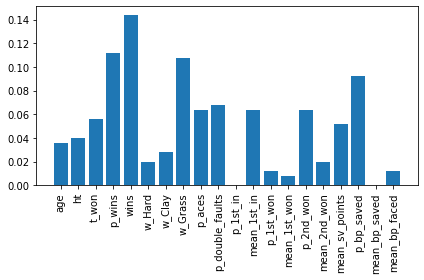
\includegraphics[width=0.35\linewidth]{images/predictive_analysis/comparison/ada_featImp_f.png}}
    \subfloat[Features importance for male]{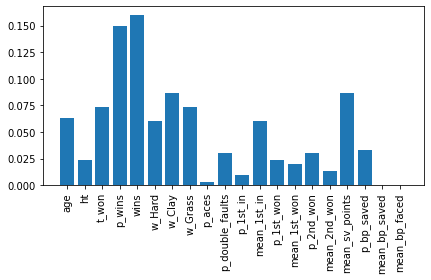
\includegraphics[width=0.35\linewidth]{images/predictive_analysis/ada_boost/ada_imp_m.png}}
    \caption{Features importance based on the sex of the player.}
    \label{fig:FeatImpSex}
\end{figure}